\documentclass[../main.tex]{subfiles}

\begin{document}
\setcounter{chapter}{3}
\chapter{Généralités sur les fonctions}
\tableofcontents
\clearpage

\setcounter{section}{20}
\section{Exemple}
On suppose que $f \geq g$. Ainsi :
\begin{align*}
    | f - g | = f - g \Leftrightarrow \frac{f + g + | f - g |}{2} = f
\end{align*}

\setcounter{section}{22}
\section{Remarque}
Soit $a \in \mathbb{Q}^*$. Soit $x \in \mathbb{R}$. 
\begin{itemize}
    \item Si $x \in \mathbb{Q}$, alors $x + a \in \mathbb{Q}$, donc $\mathds{1}_{\mathbb{Q}}(x + a) = 1 = \mathds{1}_{\mathbb{Q}}(x)$.
    \item Si $x \notin \mathbb{Q}$, alors $x + a \notin \mathbb{Q}$, donc $\mathds{1}_{\mathbb{Q}}(x + a) = 0 = \mathds{1}_{\mathbb{Q}}(x)$.
\end{itemize}

\setcounter{section}{26}
\section{Axe de symétrie}
Soit $f:I \rightarrow \mathbb{R}$ une fonction et $\mathcal{C}_f$ sa courbe représentative. \\
Soit $(x, x') \in I^2$. \\
$M$ et $M'$ sont symétriques par rapport $x = a$ \\
\noindent
\begin{minipage}[c]{0.45\textwidth}
    \begin{align*}
        &\text{ssi. }
        \begin{cases}
            a = \frac{x + x'}{2} \\[5pt]
            f(x) = f(x')
        \end{cases} \\[10pt]
        &\text{ssi. } 
        \begin{cases}
            x' = 2a - x \\[5pt]
            f(x) = f(x')
        \end{cases}
    \end{align*}
\end{minipage}
\hfill
\begin{minipage}[c]{0.45\textwidth}
\begin{tikzpicture}[x=0.75pt,y=0.75pt,yscale=-1,xscale=1]
    \draw    (155.33,145.33) -- (416.13,145.33) ; 
    \draw    (285.73,215.49) -- (285.73,45.07) ;
    \draw   (220.79,80.38) -- (220.79,80.38) -- (225.46,84.9) -- (229.98,80.24) -- (229.98,80.24) -- (225.46,84.9) -- (230.12,89.42) -- (230.12,89.42) -- (225.46,84.9) -- (220.94,89.57) -- (220.94,89.57) -- (225.46,84.9) -- cycle ;
    \draw   (340.39,80.78) -- (340.39,80.78) -- (345.06,85.3) -- (349.58,80.64) -- (349.58,80.64) -- (345.06,85.3) -- (349.72,89.82) -- (349.72,89.82) -- (345.06,85.3) -- (340.54,89.97) -- (340.54,89.97) -- (345.06,85.3) -- cycle ; 
    \draw   (225.46,84.9) -- (225.46,145.09) ;
    \draw   (345.06,85.3) -- (345.06,145.49) ;
    \draw (205.57,70.93) node [anchor=north west][inner sep=0.75pt]  [font=\tiny]  {$M( x,\ f( x))$};
    \draw (325.17,70.53) node [anchor=north west][inner sep=0.75pt]  [font=\tiny]  {$M'( x',\ f( x'))$};
    \draw (222.37,146.93) node [anchor=north west][inner sep=0.75pt]  [font=\tiny]  {$x$};
    \draw (341.17,147.33) node [anchor=north west][inner sep=0.75pt]  [font=\tiny]  {$x'$};
    \draw (290.77,207.73) node [anchor=north west][inner sep=0.75pt]  [font=\tiny]  {$a$};
\end{tikzpicture}
\end{minipage}

\section{Centre de symétrie}
On reprend les mêmes notations qu'à la $\text{(4.27)}$. \\
\noindent
\begin{minipage}[c]{0.45\textwidth}
    \begin{align*}
        &M \text{ et } M' \text{ sont symétriques par rapport à } A(a,b) \\
        &\text{ssi. } 
        \begin{cases}
            a = \frac{x + x'}{2} \\
            b = \frac{f(x) + f(x')}{2}
        \end{cases} \\
        &\text{ssi. }
        \begin{cases}
            x' = 2a - x \\
            f(x') = 2b - f(x)
        \end{cases}
    \end{align*}
\end{minipage}
\hfill
\begin{minipage}[c]{0.45\textwidth}
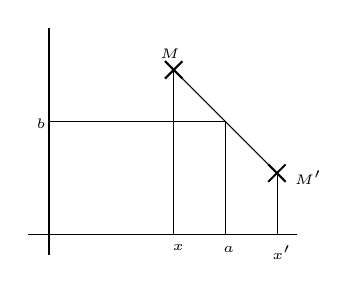
\begin{tikzpicture}[x=0.75pt,y=0.75pt,yscale=-1,xscale=1]
    \draw    (200,100.64) -- (200,209.94) ;
    \draw    (319.71,200.23) -- (190,200.23) ;
    \draw    (260.2,120.8) -- (309.89,170.49) ;
    \draw  [line width=0.75]  (255.88,116.52) -- (264.29,124.92)(264.29,116.52) -- (255.88,124.92) ;
    \draw  [line width=0.75]  (305.6,166.23) -- (314,174.64)(314,166.23) -- (305.6,174.64) ;
    \draw    (285.04,145.64) -- (285.04,199.94) ;
    \draw    (260.2,120.8) -- (260.2,200.23) ;
    \draw    (309.89,170.49) -- (309.89,199.94) ;
    \draw    (200,145.64) -- (285.04,145.64) ;
    \draw (252.4,109.48) node [anchor=north west][inner sep=0.75pt]  [font=\tiny]  {$M$};
    \draw (317.2,168.28) node [anchor=north west][inner sep=0.75pt]  [font=\tiny]  {$M'$};
    \draw (306.4,204.28) node [anchor=north west][inner sep=0.75pt]  [font=\tiny]  {$x'$};
    \draw (282.8,204.68) node [anchor=north west][inner sep=0.75pt]  [font=\tiny]  {$a$};
    \draw (258.4,203.48) node [anchor=north west][inner sep=0.75pt]  [font=\tiny]  {$x$};
    \draw (192.8,143.08) node [anchor=north west][inner sep=0.75pt]  [font=\tiny]  {$b$};
\end{tikzpicture}
\end{minipage}

\setcounter{section}{50}
\section{Exemple}
\begin{enumerate}
    \item $f'(x) = -\frac{2x + 1}{(x + x^2)^2}$
    \item $f'(x) = -\frac{1}{2x \sqrt{x}} e^\frac{1}{\sqrt{x}}$
    \item $f'(x) = -3 \frac{e^x(x-1)}{x^2} \sin \left( \frac{e^x}{x} \right) \cos^2 \left( \frac{e^x}{x} \right)$
\end{enumerate}

\section{Théorème de la bijection dérivable}
On suppose la dérivabilité de $f^{-1}$. Par définition : 
\begin{align*}
    f \circ f^{-1} = \text{Id}_I
\end{align*}
D'après la proposition $\text{(4.48.4)}$, on a :
\begin{align*}
    (f^{-1})' \circ f' \times f^{-1} &= (f \circ f^{-1})' \\ 
    &= \text{Id}_I' \\
    &= 1
\end{align*}
Comme $f$ ne s'annule pas sur $I$, on a : 
\begin{align*}
    (f^{-1})' = \frac{1}{f' \circ f^{-1}}
\end{align*}

\setcounter{section}{60}
\section{Primitives d'une fonction sur un intervalle}
\begin{itemize}
    \item Si $F$ et $G$ sont deux primitives de $f$ sur l'intervalle $I$, alors : 
    \begin{align*}
        \forall n \in I, (F - G)'(x) &= F'(x) - G'(x) \\
        &= f(x) - f(x) \\
        &= 0
    \end{align*}
    Comme $I$ est un intervalle, $F - G$ est constante $\text{(4.53)}$. \\
    Réciproquement, pour tout $a \in \mathbb{R}$, $F + a$ est aussi une primitive de $f$ sur $I$. \\

    \item Soit $G$ une primitive de $f$ sur $I$. Soit $a \in \mathbb{R}$ et $x_0 \in I$. 
    Or pour $F = G + a - G(x_0)$, $F$ est une primitve de $f$ sur $I$ et $F(x) = a$. \\
    L'unicité est donnée par le point précédent. 
\end{itemize}

\section{Exemple}
\begin{enumerate}
    \item Sur $I = \left]-\frac{\pi}{2} ; \frac{\pi}{2} \right[$. \\
    Pour tout $x \in I$, 
    \begin{align*}
        \tan x &= \frac{\sin x}{\cos x} \\
        &= -\frac{- \sin x}{\cos x}
    \end{align*}
    La primitive de $\tan$ sur $I$ est : $x \mapsto -\ln |\cos x| = \ln \cos x$.\\

    \item Sur $I = \left] -\frac{\pi}{2} ; \frac{\pi}{2} \right[$. \\
    \begin{align*}
        \forall x \in I, \tan^2 x = \tan^2 x + 1 - 1
    \end{align*}
    Une primitive de $\tan^2$ sur $I$ est : $x \mapsto \tan x - x$. \\

    \item Sur $I = \mathbb{R}$. \\
    \begin{align*}
        \forall x \in \mathbb{R}, x \sqrt{1 + x^2} &= x(1 + x^2)^{\frac{1}{2}} \\
        &= \frac{1}{2} \times 2x \times (1 + x^2)^{\frac{1}{2}} 
    \end{align*}
    Une primitive de $x \mapsto x(1 + x^2)^{\frac{1}{2}}$ sur $\mathbb{R}$ est : $x \mapsto \frac{1}{2} \times \frac{2}{3}(1 + x^2)^{\frac{3}{2}} = \frac{1}{3} (1 + x^2)^{\frac{3}{2}}$.

    \item Sur $I = \mathbb{R}_+^*$. 
    \begin{align*}
        \forall x > 0, \frac{\ln x}{x} &= \frac{1}{x} \ln x \\
    \end{align*}
    Une primitive de $x \mapsto \frac{\ln x}{x}$ sur $\mathbb{R}_+^*$ est : $x \mapsto \frac{1}{2} \ln^2 x$.
\end{enumerate}

\setcounter{section}{64}
\section{Remarque}
$G:y \mapsto y g(y) - F(g(y)) + \lambda, \lambda \in \mathbb{R}$. 
\begin{align*}
    G'(y) &= g(y) + y g'(y) - g'(y) f(g(y)) \\
    &= g(y) + \cancel{y g'(y)} - \cancel{g'(y) y} \\
    &= g(y)
\end{align*}

\section{Exemple}
\begin{align*}
    \left| \int_{-1}^{1} \frac{t^n}{1 + t^2} \,dt\ \right| &\leq \int_{-1}^{1} \frac{|t^n|}{1 + t^2} \,dt\ && \text{(Inégalité triangulaire)}\\
    &\leq \int_{-1}^{1} |t|^n \,dt\ && \text{(} \forall t, \frac{|t|^n}{1 + t^2} \leq |t|^n \text{)}\\
    &= (-1)^n \int_{-1}^{0} t^n \,dt + \int_{0}^{1} t^n \,dt\ && \text{(Relation de Chasles)}\\
    &= (-1)^n \left[ \frac{t^{n+1}}{n+1} \right]_{-1}^{0} + \left[ \frac{t^{n+1}}{n+1} \right]_{0}^{1}\ \\
    &= -\frac{(-1)^n(-1)^{n+1}}{n + 1} + \frac{1}{n + 1}\ \\
    &= \frac{2}{n + 1}
\end{align*}

\setcounter{section}{68}
\section{Intégration par partie}
\begin{align*}
    \int_{a}^{b} f'(t)g(t) \,dt + \int_{a}^{b} f(t)g'(t) \,dt &= \int_{a}^{b} (f'(t)g(t) + f(t)g'(t)) \,dt \\
    &= \int_{a}^{b} (fg)'(t) \,dt \\
    &= [f(t)g(t)]_{a}^{b} 
\end{align*}

\section{Changement de variable}
Comme $f$ est une fonction continue sur $[a,b]$, on choisit une primitive $F$ de $f$ sur $[a,b]$. $\text{(Théorème fondamental du calcul intégral)}$ \\
Ainsi : 
\begin{align*}
    \int_{u(a)}^{u(b)} f(t) \,dt &= \left[ F(t) \right]_{u(a)}^{u(b)} \\
    &= F \circ u(b) - F \circ u(a) \\
\end{align*}
Or : 
\begin{align*}
    \int_{a}^{b} f(u(t))u'(t) \,dt &= \int_{a}^{b} F'(u(t)) \times u'(t) \,du(t) \\
    &= \left[ F \circ u(t) \right]_a^b 
\end{align*}

\setcounter{section}{71}
\section{Exemple}
Si $x = \sin t$, alors $dx = \cos t \,dt$. \\
Pour $t = 0$, $x = \sin 0 = 0$. \\
Pour $t = \frac{\pi}{2}$, $x = \sin \frac{\pi}{2} = 1$. \\
Or $t \mapsto \sin t \in \mathcal{C}^1(\left[0 ; \frac{\pi}{2}\right], \mathbb{R})$. \\
D'après le théorème de changement de variable : 
\begin{align*}
    \int_{0}^{1} \sqrt{1 - x^2} \,dx &= \int_{0}^{\frac{\pi}{2}} \sqrt{1 - \sin^2 t} \cos t \,dt\ \\
    &= \int_{0}^{\frac{\pi}{2}} \sqrt{\cos^2 t} \cos t \,dt\ \\ 
    &= \int_{0}^{\frac{\pi}{2}} \cos^2 t \,dt\ \\
    &= \int_{0}^{\frac{\pi}{2}} \frac{1 + \cos 2t}{2} \,dt\ \\
    &= \left[\frac{1}{4} \sin 2t \right]_{0}^{\frac{\pi}{2}} + \frac{\pi}{4} \\
    &= \frac{\pi}{4} 
\end{align*}

\setcounter{section}{73}
\section{Méthode}
Pour tout $x \in \mathbb{R}\backslash \{ a ; b\}$, trouver $c$ et $d$ tel que $\frac{\alpha x + \beta}{(x - a)(x - b)} = \frac{c}{x-a} + \frac{d}{x - b}$ : 
\begin{align*}
    \frac{\alpha x + \beta}{(x - b)} &= c + \frac{d(x - a)}{(x - b)} && \text{(On multiplie par $(x - a)$)} \\
    c &= \frac{\alpha a + \beta}{a - b} && \text{($x = a$)} \\
    d &= \frac{\alpha b + \beta}{b - a} && \text{($x = b$)}
\end{align*}

\section{Exemple}
\begin{align*}
    f:x \mapsto \frac{2x - 1}{(x + 1)(x - 3)} = \frac{4}{3(x+1)} + \frac{4}{5(x - 3)}
\end{align*}
Une primitive de $f$ sur $]-1 ; 3[$ est : $x \mapsto \frac{3}{4} \ln |x + 1| + \frac{5}{4} \ln |x - 3| = \frac{3}{4} \ln (x + 1) + \frac{5}{4} \ln (x - 3)$

\end{document}